\documentclass[12pt, a4paper]{report}
\usepackage{graphicx, array, amsthm, amssymb, amsmath, algorithm, algpseudocode, float, xcolor, thmtools, thmbox, exercise}
\usepackage[english]{babel}

\makeatletter
\renewcommand\thmbox@headstyle[2]{\bfseries #1}
\makeatother
\newtheorem[style=M,bodystyle=\normalfont]{theorem}{Theorem}
\newtheorem[style=M,bodystyle=\normalfont]{corollary}{Corollary}
\newtheorem[style=M,bodystyle=\normalfont]{lemma}{Lemma}
\newtheorem[style=M,bodystyle=\normalfont]{definition}{Definition}


\title{Data Bases II \\ \textit{Exercises}}
\author{Christian Rossi}
\date{Academic Year 2023-2024}

\begin{document}

\maketitle

\newpage

\begin{abstract}
    The course aims to prepare software designers on the effective development of database applications. 
    
    First, the course presents the fundamental features of current database architectures, with a specific emphasis on the concept of transaction and its realization in centralized 
    and distributed systems. 
    
    Then, the course illustrates the main directions in the evolution of database systems, presenting approaches that go beyond the relational model, like active databases, object 
    systems and XML data management solutions.
\end{abstract}

\newpage

\tableofcontents

\newpage

\chapter{Exercise session I}
    \section{Anomalies classification}
        Can the following schedules produce anomalies? $c_i$ and $a_i$ indicate the transactional decision commit and abort. 
        \begin{enumerate}
            \item $r_1(x) w_1(x) r_2(x) w_2(y)\:a_1\:c_2$
            \item $r_1(x) w_1(x) r_2(y) w_2(y)\:a_1\:c_2$
            \item $r_1(x) r_2(x) r_2(y) w_2(y) r_1(z)\:a_1\:c_2$
            \item $r_1(x) r_2(x) w_2(x) w_1(x)\:c_1\:c_2$
            \item $r_1(x) r_2(x) w_2(x) r_1(y)\:c_1\:c_2$
            \item $r_1(x) w_1(x) r_2(x) w_2(x)\:c_1\:c_2$
        \end{enumerate}
    \subsection*{Solution}
        \begin{enumerate}
            \item We have a serial execution, but with the abort of the first transaction. Since the second transaction reads the modified value of $x$ before the abort, we have a
                dirty read. 
            \item We have a serial execution and the two transactions require different resources, so there are no anomalies.
            \item There are no anomalies because the last operation of the first transaction works on a different resource. 
            \item Both transactions first reads in sequence the resource $x$ and then updates it without considering the updated value, so we have a lost update. 
            \item There are no anomalies because the last operation of the first transaction works on a different resource. 
            \item We have a serial execution, so the schedule is correct. 
        \end{enumerate}

    \newpage

    \section{Anomalies classification}
        The following schedule may produce 2 anomalies: a lost update and a phantom update. Identify them. 
        \[r_1(x) r_2(x) r_3(x) w_1(x) r_4(y) w_2(x) r_4(x) w_4(y) r_3(y)w_4(x) r_5(y) w_6(y) w_5(y) w_7(y)\]
    \subsection*{Solution}
        We can write the schedule in the following way:
        \begin{table}[H]
            \centering
            \resizebox{\textwidth}{!}{%
            \begin{tabular}{cccccccccccccc}
            $r_1(x)$           &           &                    & $w_1(x)$           & \textbf{} & \textbf{} & \textbf{} & \textbf{} & \textbf{} & \textbf{} & \textbf{} & \textbf{} & \textbf{} & \textbf{} \\
                            & $r_2(x)$  & \textit{\textbf{}} & \textit{\textbf{}} & \textbf{} & $w_2(x)$  & \textbf{} & \textbf{} & \textbf{} & \textbf{} & \textbf{} & \textbf{} & \textbf{} & \textbf{} \\
            \textit{\textbf{}} & \textbf{} & $r_3(x)$           & \textbf{}          & \textbf{} & \textbf{} & \textbf{} & \textbf{} & $r_3(y)$  & \textbf{} & \textbf{} & \textbf{} & \textbf{} & \textbf{} \\
            \textit{\textbf{}} & \textbf{} & \textbf{}          &                    & $r_4(y)$  & \textbf{} & $r_4(x)$  & $w_4(y)$  & \textbf{} & $w_4(x)$  & \textbf{} & \textbf{} & \textbf{} & \textbf{} \\
            \textit{\textbf{}} & \textbf{} & \textbf{}          & \textbf{}          & \textbf{} & \textbf{} & \textbf{} & \textbf{} & \textbf{} & \textbf{} & $r_5(y)$  & \textbf{} & $w_5(y)$  & \textbf{} \\
            \textbf{}          & \textbf{} & \textbf{}          & \textbf{}          & \textbf{} & \textbf{} & \textbf{} & \textbf{} & \textbf{} & \textbf{} & \textbf{} & $w_6(y)$  & \textbf{} & \textbf{} \\
            \textbf{}          & \textbf{} & \textbf{}          & \textbf{}          & \textbf{} & \textbf{} & \textbf{} & \textbf{} & \textbf{} & \textbf{} & \textbf{} & \textbf{} & \textbf{} & $w_7(y)$ 
            \end{tabular}%
            }
        \end{table}
        And we can see that there is a lost update with transactions $T_1$ and $T_2$ and a phantom update with $T_3$ and $T_4$. 

    \newpage
    
    \section{Schedule classification}
        Classify the following schedule with respect to CSR and VSR classes: 
        \[r_1(x) r_2(y) w_3(y) r_5(x) w_5(u) w_3(s)w_2(u) w_3(x) w_1(u) r_4(y) w_5(z) r_5(z)\]
    \subsection*{Solution}
        Since CSR contains VSR we check with the conflict graph. To do so we first divide the schedule based on the resources: 
        \begin{itemize}
            \item $x: r_1 \: r_5 \:w_3$
            \item $y: r_2 \: w_3 \:r_4$
            \item $z: w_5 \: r_5$
            \item $s: w_3$
            \item $u: w_5 \: w_2 \:w_1$
        \end{itemize}
        The nodes are $\{1,2,3,4,5\}$ and the arcs are found with the write-write or write-read relations found in the previous groups. 
        So we have the following graph:
        \begin{figure}[H]
            \centering
            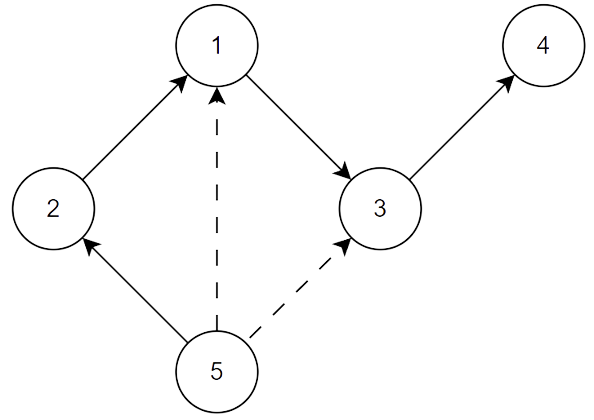
\includegraphics[width=0.5\linewidth]{images/conflictgraph.png}
        \end{figure}
        Some arcs can be omitted if the nodes are connected in another way (in this case we can remove arcs $\{\{5,1\},\{5,3\}\}$). 

        There are no cycles: the schedule is CSR (and also VSR). 

    \newpage
    
    \section{Schedule classification}
        Classify the following schedule with respect to CSR and VSR classes:  
        \[r_2(u) w_2(s) r_1(x) r_2(y) w_3(y) r_5(x) w_5(u) w_3(s)w_2(u) w_3(x) w_1(u) r_4(y) w_5(z) r_5(z)\]
    \subsection*{Solution}
        Since CSR contains VSR we check with the conflict graph. To do so we first divide the schedule based on the resources: 
        \begin{itemize}
            \item $x: r_1 \: r_5 \:w_3$
            \item $y: r_2 \: w_3 \:r_4$
            \item $z: w_5 \: r_5$
            \item $s: w_2 \: w_3$
            \item $u: r_2 \: w_5 \: w_2 \:w_1$
        \end{itemize}
        The nodes are $\{1,2,3,4,5\}$ and the arcs are found with the write-write or write-read relations found in the previous groups. So we have the following graph:
        \begin{figure}[H]
            \centering
            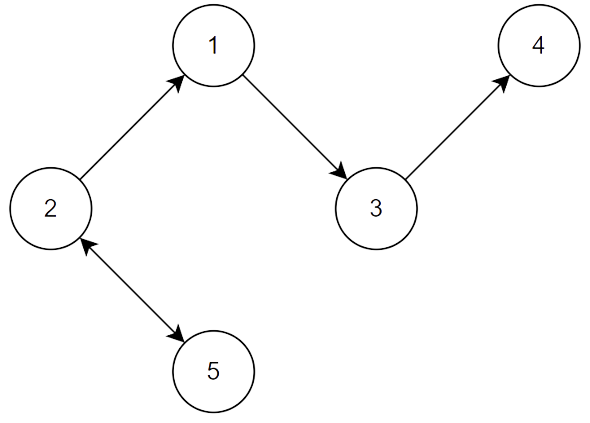
\includegraphics[width=0.5\linewidth]{images/conflictgraph1.png}
        \end{figure}
        It is possible to see that there is a cycle between two and five. The definition of VSR states that we need to have the same reads-from relations and final writes. So, we try to find a view-equivalent 
        schedule that is also CSR. One possible solution is simply to swap the two writes on the resource $u$ and that is sufficient to eliminate the cycle. So, the schedule: 
        \[r_2(u) w_2(s) r_1(x) r_2(y) w_3(y) r_5(x) w_5(u) w_2(u) w_3(s) w_3(x) w_1(u) r_4(y) w_5(z) r_5(z)\]
        is CSR and also VSR. 

    \newpage
    
    \section{Schedule classification}
        Classify the following schedule with respect to CSR and VSR classes:  
        \[r_1(x) r_2(y) w_3(y) r_5(x) w_5(u) w_3(s)w_2(u) w_3(x) w_1(u) r_4(y) w_5(z) r_5(z) r_2(u) w_2(s)\]
    \subsection*{Solution}
        Since CSR contains VSR we check with the conflict graph. To do so we first divide the schedule based on the resources: 
        \begin{itemize}
            \item $x: r_1 \: r_5 \: w_3$
            \item $y: r_2 \: w_3 \: r_4$
            \item $z: w_5 \: r_5$
            \item $s: w_3 \: w_2$
            \item $u: w_5 \: w_2 \: w_1 \: r_2$
        \end{itemize}
        The nodes are $\{1,2,3,4,5\}$ and the arcs are found with the write-write or write-read relations found in the previous groups. So we have the following graph:
        \begin{figure}[H]
            \centering
            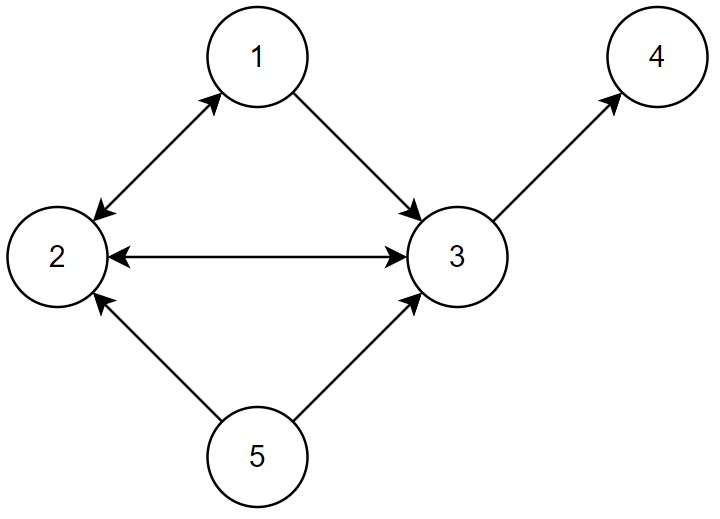
\includegraphics[width=0.5\linewidth]{images/conflictgraph2.png}
        \end{figure}
        In this case it is not possible to find a VSR schedule because it is impossible to do so without changing the final write on $s$. 

    \newpage

    \section{Schedule classification}
        Classify the following schedule with respect to CSR and VSR classes:  
        \[r_5(x) r_3(y) w_3(y) r_6(t) r_5(t) w_5(z) w_4(x) r_3(z) w_1(y) \dots\]
        \[\dots r_6(y) w_6(t) w_4(z) w_1(t) w_3(x) w_1(x) r_1(z) w_2(t) w_2(z)\]
    \subsection*{Solution}
        Since CSR contains VSR we check with the conflict graph. To do so we first divide the schedule based on the resources: 
        \begin{itemize}
            \item $t: \: r_6 \: r_5 \: w_6 \: w_1 \: w_2$
            \item $x: \: r_5 \: w_4 \: w_3 \: w_1$
            \item $y: \: r_3 \: w_3 \: w_1 \: r_6$
            \item $z: \: w_5 \: r_3 \: w_4 \: r_1 \: w_2$
        \end{itemize}
        The nodes are $\{1,2,3,4,5,6\}$ and the arcs are found with the write-write or write-read relations found in the previous groups. So we have the following graph:
        \begin{figure}[H]
            \centering
            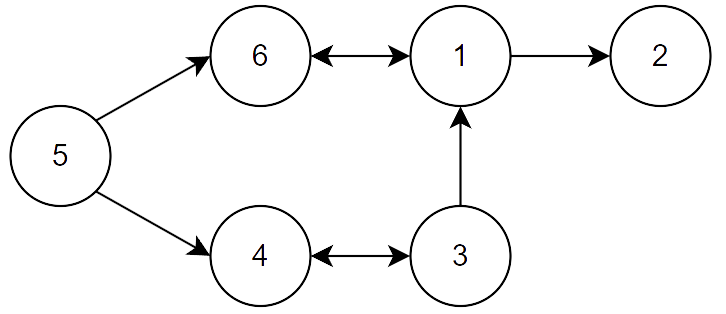
\includegraphics[width=0.5\linewidth]{images/conflictgraph3.png}
        \end{figure}
        We have two cycles. It is impossible to find a VSR schedule because only the conflict between four and three can be eliminated (the other one changes a read-write relation).

    \newpage

    \chapter{Exercise session II}
    \section{Schedule classification}
        Classify the following schedule with respect to 2PL and strict 2PL classes: 
        \[r_1(x) r_2(y) w_3(y) r_5(x) w_5(u) w_3(s) w_2(u) w_3(x) w_1(u) r_4(y) w_5(z) r_5(z)\]
    \subsection*{Solution}
        For strict 2PL we assume that all transactions commit and release all locks immediately after their last operation, and check if releases can be executed at commit time.
        \begin{table}[H]
            \centering
            \resizebox{\columnwidth}{!}{%
            \begin{tabular}{c|cccccccccccc}
                    & \textit{1} & \textit{2}      & \textit{3} & \textit{4} & \textit{5} & \textit{6} & \textit{7}                        & \textit{8}      & \textit{9}              & \textit{10} & \textit{11} & \textit{12}             \\ \hline
            \textit{S} &            &                 &            &            &            & $w_3$      &                                   &                 &                         &             &             &                         \\
            \textit{U} &            &                 &            &            & $w_5$      &            & $\searrow_5w_2\downharpoonleft_2$ &                 & $w_1\downharpoonleft_1$ &             &             &                         \\
            \textit{X} & $r_1$      &                 &            & $r_5$      &            &            &                                   & $\searrow_1w_3$ &                         &             &             &                         \\
            \textit{Y} &            & $r_2\searrow_2$ & $w_3$      &            &            &            &                                   &                 &                         & $r_4$       &             &                         \\
            \textit{Z} &            &                 &            &            &            &            &                                   &                 &                         &             & $w_5$       & $r_5\downharpoonleft_5$
            \end{tabular}%
            }
        \end{table}
        $S$ clearly cannot be in strict 2PL. The contradictions are:
        \begin{itemize}
            \item $T_1$ must release $X$ before $8$. 
            \item $T_2$ must release $Y$ before $7$.
            \item $T_5$ must release $U$ before $12$.
        \end{itemize}
        For 2PL we have:
        \begin{table}[H]
            \centering
            \resizebox{\columnwidth}{!}{%
            \begin{tabular}{c|cccccccccccc}
                    & \textit{1} & \textit{2}      & \textit{3} & \textit{4} & \textit{5} & \textit{6} & \textit{7}                        & \textit{8}      & \textit{9}              & \textit{10} & \textit{11} & \textit{12}             \\ \hline
            \textit{S} &                            &                                   &                           &                           &                           & $\nearrow_3w_3$       &                                       & $\searrow_3$                          &                         &                             &             &                         \\
            \textit{U} &                            &                                   &                           &                           & $\nearrow_5w_5\searrow_5$ &                       & $\nearrow_2w_2\searrow_2\nearrow_1$   &                                       & $w_1\searrow_1$         &                             &             &                         \\
            \textit{X} & $\nearrow_1r_1$            &                                   &                           & $\nearrow_5r_5$           &                           & $\searrow_5$          &                                       & $\searrow_1\nearrow_3w_3\searrow_3$   &                         &                             &             &                         \\
            \textit{Y} &                            & $\nearrow_2r_2\searrow_2$         & $\nearrow_3w_3$           &                           &                           &                       &                                       &                                       & $\searrow_3$            & $\nearrow_4r_4\searrow_4$   &             &                         \\
            \textit{Z} &                            &                                   &                           & $\nearrow_5$              &                           &                       &                                       &                                       &                         &                             & $w_5$       & $r_5\searrow_5$
            \end{tabular}%
            }
        \end{table}
        It is also not in 2PL: an assignment is not possible for $T_2$ (which must release $Y$ before locking $U$).

    \newpage

    \section{Schedule classification}
        Classify the following schedule with respect to 2PL and strict 2PL classes: 
        \[r_4(x) r_2(x) w_4(x) w_2(y) w_4(y) r_3(y) w_3(x) w_4(z) r_3(z) r_6(z) r_8(z) w_6(z) w_9(z) r_5(z) r_10(z)\]
    \subsection*{Solution}
        For strict 2PL we assume that all transactions commit and release all locks immediately after their last operation, and check if releases can be executed at commit time.
        \begin{table}[H]
            \centering
            \resizebox{\columnwidth}{!}{%
            \begin{tabular}{c|ccccccccccccccc}
                       & \textit{1} & \textit{2} & \textit{3} & \textit{4} & \textit{5} & \textit{6} & \textit{7} & \textit{8} & \textit{9} & \textit{10} & \textit{11} & \textit{12} & \textit{13} & \textit{14} & \textit{15} \\ \hline
            \textit{X} & $r_4$      & $r_2\searrow _2$          & $w_4$      &                              &            &            & $w_3$      &            &            &             &             &             &             &             &             \\
            \textit{Y} &            &                           &            & $w_2\downharpoonleft_2$      & $w_4$      & $r_3$      &            &            &            &             &             &             &             &             &             \\
            \textit{Z} &            &                           &            &                              &            &            &            & $w_4$      & $r_3$      & $r_6$       & $r_8$       & $w_6$       & $w_9$       & $r_5$       & $r_{10}$     
            \end{tabular}%
            }
        \end{table}
        It is therefore clear that the schedule cannot be in 2PL-strict, due to $T_2$ and $T_4$: $T_2$ ends after 4, but $T_4$ wants to write $X$ at 3, and $T_2$ would thus be 
        required to release $X$ earlier, which is impossible if $T_2$ has to keep all locks until after 4.

        For 2PL we have:
        \begin{table}[H]
            \centering
            \resizebox{\columnwidth}{!}{%
            \begin{tabular}{c|ccccccccccccccc}
                       & \textit{1} & \textit{2} & \textit{3} & \textit{4} & \textit{5} & \textit{6} & \textit{7} & \textit{8} & \textit{9} & \textit{10} & \textit{11} & \textit{12} & \textit{13} & \textit{14} & \textit{15} \\ \hline
            \textit{X} & $\nearrow_4r_4$        & $\nearrow_2r_2\searrow_2$         & $\nearrow_4w_4$       &                       & $\searrow_4$                          &                           & $\nearrow_3w_3$       &                       &                          & $\searrow_3$  &                       &             &             &             &             \\
            \textit{Y} &                        & $\nearrow_2$                      &                       & $w_2\searrow_2$       & $\nearrow_4w_4\searrow_4$             & $\nearrow_3r_3$           &                       &                       &                          & $\searrow_3$  &                       &             &             &             &             \\
            \textit{Z} &                        &                                   & $\nearrow_4$          &                       &                                       &                           &                       & $w_4\searrow_4$       & $\nearrow_3r_3$          & $r_6$         & $r_8\searrow_3$       & $w_6$       & $w_9$       & $r_5$       & $r_{10}$     
            \end{tabular}%
            }
        \end{table}
        We need to look at those acquisitions that must be anticipated and to those releases that must be delayed to not violate the 2PL rules.
        $T_4$ can only get the XL on X only after 2 and on $Y$ after 4 and has to release $Y$ before 6 and $X$ before 7. Thus, the lock on $Z$ must be acquired before 6.
        $T_2$ can get all the locks at the beginning and release them immediately after each use. $T_3$ can acquire $X$, $Y$ and $Z$ just before using them and release them all before 12. 
        All other transactions ($T_6, T_9, T_5, T_10$) clearly pose no problems.

    \newpage

    \section{Schedule classification}
        Classify the following schedule with respect to 2PL and strict 2PL classes: 
        \[r_1(A) r_2(A) w_2(A) r_1(B) w_1(C) w_2(C) r_3(C) w_3(A) w_2(B) w_3(B)\]
    \subsection*{Solution}
        For strict 2PL we assume that all transactions commit and release all locks immediately after their last operation, and check if releases can be executed at commit time.
        \begin{table}[H]
            \centering
            \resizebox{\columnwidth}{!}{%
            \begin{tabular}{c|cccccccccc}
                    & \textit{1} & \textit{2} & \textit{3} & \textit{4} & \textit{5} & \textit{6} & \textit{7} & \textit{8} & \textit{9} & \textit{10} \\ \hline
            \textit{A} & $r_1$      & $r_2\searrow _1$          & $w_2$      &            &            &            &            & $w_3$      &            &             \\
            \textit{B} &            &                           &            &            & $w_1\downharpoonleft_1$      & $w_2$      & $r_3$      &            &            &             \\
            \textit{C} &            &                           &            & $r_1$      &            &            &            &            & $w_2$      & $w_3$      
            \end{tabular}%
            }
        \end{table}
        The schedule is not strict 2PL.

        For 2PL we have:
        \begin{table}[H]
            \centering
            \resizebox{\columnwidth}{!}{%
            \begin{tabular}{c|cccccccccc}
                    & \textit{1} & \textit{2} & \textit{3} & \textit{4} & \textit{5} & \textit{6} & \textit{7} & \textit{8} & \textit{9} & \textit{10} \\ \hline
            \textit{A} & $\nearrow_1r_1$        & $\nearrow_2r_2\searrow_1$         & $\nearrow_2w_2$       &                   &                   & $\searrow_2$                      &                           & $\nearrow_3w_3$       &                       & $\searrow_3$            \\
            \textit{B} &                        & $\nearrow_1$                      &                       &                   & $w_1\searrow_1$   & $\nearrow_2w_2\searrow_2$         & $\nearrow_3r_3$           &                       &                       & $\searrow_3$            \\
            \textit{C} &                        & $\nearrow_1$                      &                       & $r_1\searrow_1$   &                   &                                   &                           &                       & $w_2\searrow_2$       & $\nearrow_3w_3\searrow_3$      
            \end{tabular}%
            }
        \end{table}
        The schedule is 2PL. 

    \newpage

    \section{Schedule classification}
        Classify the following schedule with respect to 2PL and strict 2PL classes: 
        \[r_1(x) w_2(x) r_1(z) w_1(y) r_3(x) r_4(x) w_3(z) w_2(y) r_3(y) w_4(x) w_4(y)\]
    \subsection*{Solution}
        For strict 2PL we assume that all transactions commit and release all locks immediately after their last operation, and check if releases can be executed at commit time.
        \begin{table}[H]
            \centering
            \resizebox{\columnwidth}{!}{%
            \begin{tabular}{c|ccccccccccc}
                       & \textit{1} & \textit{2} & \textit{3} & \textit{4} & \textit{5} & \textit{6} & \textit{7} & \textit{8} & \textit{9} & \textit{10} & \textit{11}          \\ \hline
            \textit{X} & $r_1\searrow_1$       & $w_2$      &            &                                  & $r_3$      & $r_4$      &            &            &            & $w_4$       &                    \\
            \textit{Y} &                       &            &            & $w_1\downharpoonleft_1$          &            &            &            & $w_2$      & $r_3$      &             & $w_4$                \\
            \textit{Z} &                       &            & $r_1$      &                                  &            &            & $w_3$      &            &            &             &                     
            \end{tabular}%
            }
        \end{table}
        The schedule is not strict 2PL.

        For 2PL we have:
        \begin{table}[H]
            \centering
            \resizebox{\columnwidth}{!}{%
            \begin{tabular}{c|ccccccccccc}
                       & \textit{1} & \textit{2} & \textit{3} & \textit{4} & \textit{5} & \textit{6} & \textit{7} & \textit{8} & \textit{9} & \textit{10} & \textit{11}          \\ \hline
            \textit{X} & $\nearrow_1r_1\searrow_1$              & $\nearrow_2w_2$       &                       &                                   & $\searrow_2\nearrow_3r_3$         & $\nearrow_4r_4$       &                       &                   & $\searrow_3$                   & $\nearrow_4w_4$       & $\searrow_4$     \\
            \textit{Y} & $\nearrow_1$                           &                       &                       & $w_1\searrow_1\nearrow_2$         &                                   &                       &                       & $w_2\searrow_2$   & $\nearrow_3r_3\searrow_3$      &                       & $\nearrow_4w_4\searrow_4$                \\
            \textit{Z} & $\nearrow_1$                           &                       & $r_1\searrow_1$       &                                   &                                   &                       & $\nearrow_3w_3$       &                   & $\searrow_3$                   &                       &                     
            \end{tabular}%
            }
        \end{table}
        The schedule is 2PL. 

    \newpage

    \section{Update locks}
        Given the schedule:
        \[r1(x) r2(x) r3(y) w3(y) w1(x) w2(y)\]
        show the sequence of lock and unlock requests produced by the transactions in a 2PL execution, in a system with update lock (available locks: $SL, UL, XL$).
    \subsection*{Solution}
        The locking phases with update locks are the following: 
        \begin{table}[H]
            \centering
            \begin{tabular}{|c|c|}
            \hline
            $X$                                           & $Y$                                           \\ \hline
            $\textnormal{UL}_1(x)$                        &                                               \\
            $r_1(x)$                                      &                                               \\
            $\textnormal{SL}_2(x)$                        &                                               \\
            $r_2(x)$                                      &                                               \\
                                                          & $\textnormal{UL}_3(y)$                        \\
                                                          & $r_3(y)$                                      \\
                                                          & $\textnormal{XL}_3(y) [\textnormal{upgrade}]$ \\
                                                          & $w_3(y)$                                      \\
                                                          & $\textnormal{rel}(\textnormal{XL}_3(y))$      \\
                                                          & $\textnormal{XL}_2(y)$                        \\
            $\textnormal{rel}(\textnormal{SL}_2(x))$      &                                               \\
            $\textnormal{XL}_1(x) [\textnormal{upgrade}]$ &                                               \\
            $w_1(x)$                                      &                                               \\
            $\textnormal{rel}(\textnormal{XL}_1(x))$      &                                               \\
                                                          & $w_2(y)$                                      \\
                                                          & $\textnormal{rel}(\textnormal{XL}_2(y))$      \\ \hline
            \end{tabular}
        \end{table}

    \newpage

    \section{Update locks}
        Update lock was introduced to contrast deadlocks. Can we state that deadlocks are impossible in the presence of update locks?
        \begin{enumerate}
            \item If so, concisely explain why. 
            \item If not, provide a counter-example.
        \end{enumerate}
    \subsection*{Solution}
        \begin{enumerate}
            \item Clearly deadlocks are possible in the presence of UL. Indeed, UL only makes deadlock less likely, by preventing one type of deadlock, due to 
                update patterns, when two transactions compete for the same resource ($r_1(x) r_2(x) w_1(x) w_2(x)$). 
            \item Consider two distinct resources $X$ and $Y$, and two transactions that want to access them in this order: $r_1(X) r_2(Y) w_1(Y) w_2(X)$. It is likely that they end up 
                in deadlock, especially if the system on which they run applies 2PL. UL is totally irrelevant here, because there is no update pattern. 
        \end{enumerate}

\newpage

\chapter{Exercise session III}
    \section{Obermarck's algorithm}
        Consider the following waiting conditions:
        \begin{itemize}
            \item Node $A$: $E_B \rightarrow t_1, t_1 \rightarrow t_2, E_C \rightarrow t_2, t_2 \rightarrow t_3, t_3 \rightarrow E_B, E_B \rightarrow t_4, t_4 \rightarrow t_3$
            \item Node $B$: $E_A \rightarrow t_3, t_3 \rightarrow t_5, t_5 \rightarrow t_6, t_6 \rightarrow E_C, E_C \rightarrow t_7, t_7 \rightarrow t_6, t_9 \rightarrow t_4,t_4 \rightarrow E_A, t_1 \rightarrow E_A$
            \item Node $C$: $E_B \rightarrow t_6, t_6 \rightarrow t_8, t_8 \rightarrow t_2, t_2 \rightarrow E_A, t_7 \rightarrow E_B$
        \end{itemize}
        Simulate the Obermarck algorithm and indicate whether there is a distributed deadlock.
    \subsection*{Solution}
        We need to construct the graph with the given constraints, that is: 
        \begin{figure}[H]
            \centering
            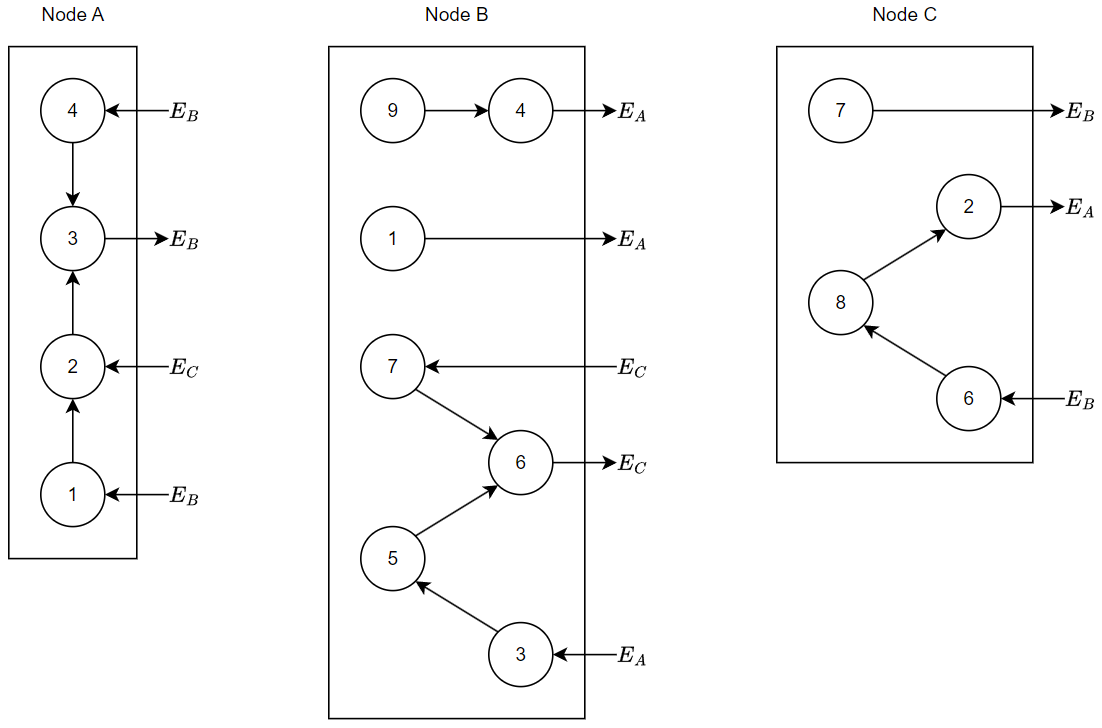
\includegraphics[width=0.75\linewidth]{images/Ob1.png}
        \end{figure}
        We have to check all the nodes where the sender has a lower value than the receiver. In this case we have that the update is sent to the 
        other distributed node. The interesting cases are highlighted in the image. So, we now have to add the nodes: 
        \begin{itemize}
            \item $4 \rightarrow 3$ in $E_B$. 
            \item $7 \rightarrow 6$ in $E_C$. 
            \item $6 \rightarrow 2$ in $E_A$. 
        \end{itemize}
        If the numbered node is not present we can add it to the graph of the distributed node. We obtain the following graphs: 
        \begin{figure}[H]
            \centering
            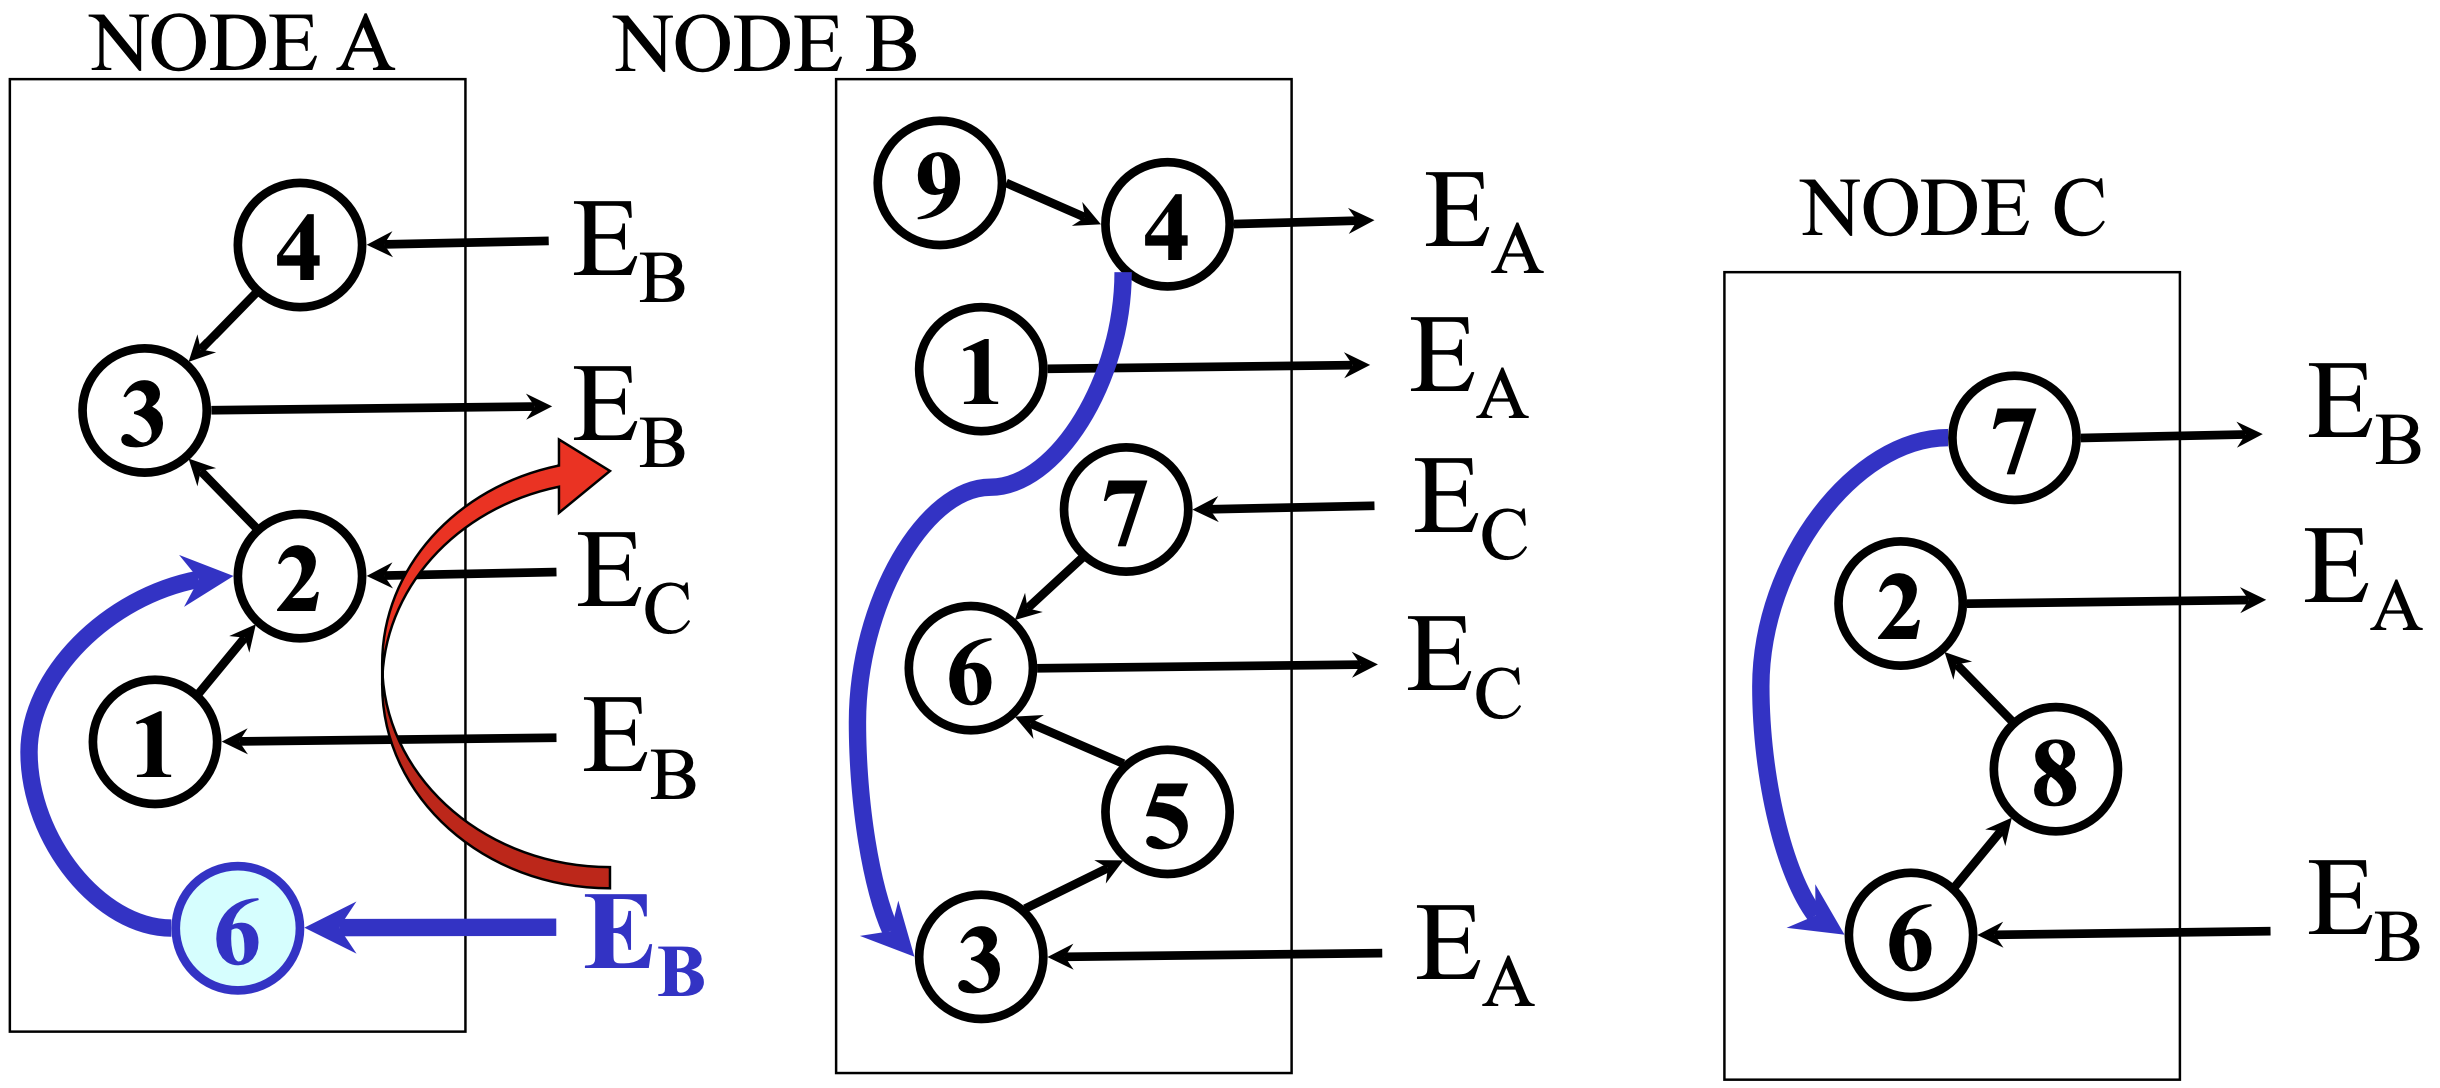
\includegraphics[width=0.75\linewidth]{images/Ob2.png}
        \end{figure}
        We have to check if other messages are sent. We have:
        \begin{itemize}
            \item $6 \rightarrow 3$ in $E_B$. 
        \end{itemize}
        So the updated graph is: 
        \begin{figure}[H]
            \centering
            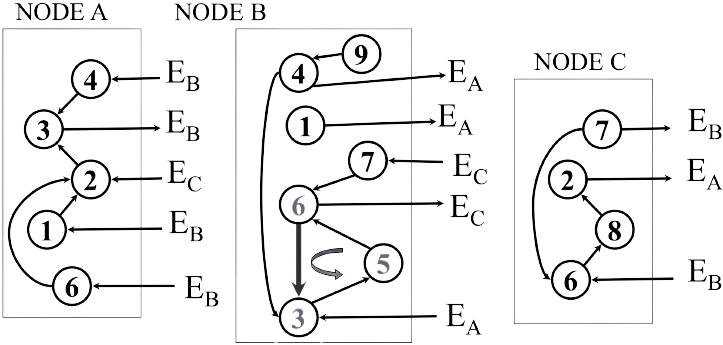
\includegraphics[width=0.75\linewidth]{images/Ob3.png}
        \end{figure}
        We have found find a cycle, so there is a deadlock. 

    \newpage

    \section{Obermarck's algorithm}
        The nodes $A$, $B$, and $C$ of a distributed transactional system are aware of the following remote and local waiting conditions:
        \begin{itemize}
            \item Node $A: E_B \rightarrow t_3, E_C \rightarrow t_2, t_1 \rightarrow E_C, t_3 \rightarrow t_5, t_5 \rightarrow t_1$
            \item Node $B: E_C \rightarrow t_2, t_3 \rightarrow E_A, t_2 \rightarrow t_3$
            \item Node $C: t_2 \rightarrow E_A, t_2 \rightarrow E_B, t_1 \rightarrow t_4, t_4 \rightarrow t_2$
        \end{itemize}
        Execute the Obermarck's algorithm twice, with different conventions:
        \begin{enumerate}
            \item Sending messages of the form $E_X \rightarrow t_i \rightarrow t_j \rightarrow E_Y$ forward (toward node $Y$) and only 
                if and only if $i > j$. 
            \item With the opposite conventions, so if and only if $i > j$
        \end{enumerate}
        Discuss the outcome, and explain it, taking into account the properties of the algorithm and the initial conditions.
    \subsection*{Solution}
        The graph is the following: 
        \begin{figure}[H]
            \centering
            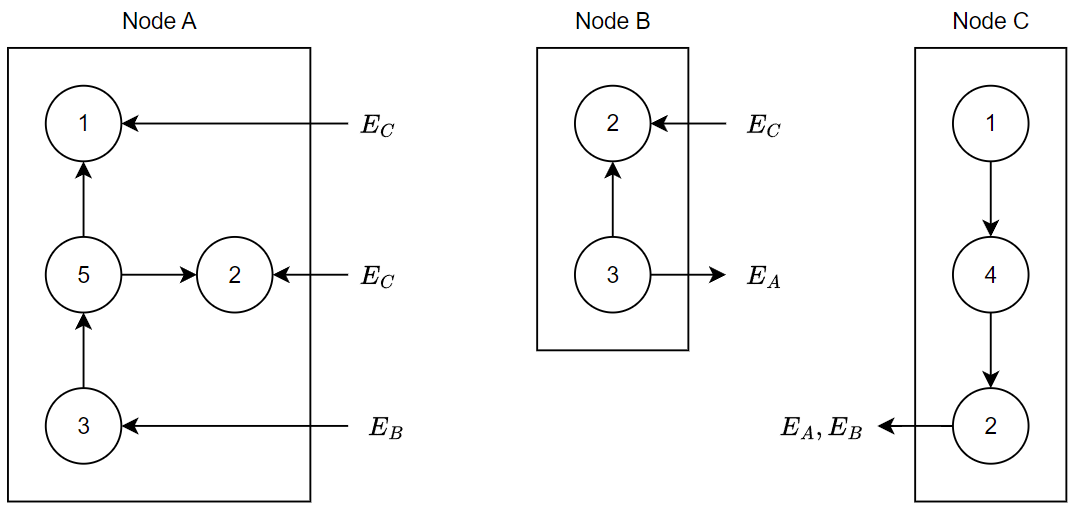
\includegraphics[width=0.75\linewidth]{images/Ob4.png}
        \end{figure}
        \begin{enumerate}
            \item We have to add the nodes (connections are distributed): 
                \begin{itemize}
                    \item $3 \rightarrow 1$ in $E_C$. 
                    \item $3 \rightarrow 2$ in $E_A$. 
                    \item $3 \rightarrow 2$ in $E_B$. 
                \end{itemize}
                By adding those nodes we found that the third one creates a deadlock. 
            \item We have to add the node (connections are distributed): 
                \begin{itemize}
                    \item $2 \rightarrow 3$ in $E_A$. 
                \end{itemize}
                No cycles are found, so no deadlocks found. 
        \end{enumerate}
        The algorithm is independent of the conventions but the initial conventions, but the initial conditions must be consistent and complete. 
        On a faulty dataset even the best algorithm returns untrustworthy results. In this case we have a link missing between node $A$ and $C$.

    \newpage

    \section{Schedule classification}
        Classify the following schedule with respect to timestamps: 
        \[r_4(x) r_2(x) w_4(x) w_2(y) w_4(y) r_3(y) w_3(x) w_4(z) r_3(z) r_6(z) r_8(z) w_6(z) w_9(z) r_5(z) r_{10}(z)\]
    \subsection*{Solution}
        We can identify pairs of operations that cause killings:
        \begin{itemize}
            \item $X: r_4 r_2 w_4 w_3$
            \item $Y: w_2 w_4 r_3$
            \item $Z: w_4 r_3 r_6 r_8 w_6 w_9 r_5 r_{10}$
        \end{itemize}
        On $X$ we have that $w_3$ is too late with respect to $r_4$ and $w_4$. On $Y$ we have that $r_3$ is late with respect to $w_4$. On 
        $Z$ we have that $r_3$ is late with respect to $w_4$, $w_6$ with respect to $r_8$, $r_5$ with respect to both $w_6$ and $w_9$. 
        So, the schedule is not in TS-mono. 

        The schedule is also outside TS-multi, because $w_3(X)$ comes too late ($r_4(X)$ was already given the initial version instead) and 
        also because $w_6(Z)$ is late with respect to r$8(Z)$. The other five reasons were due to reads (that are always accepted in TS-multi).

    \newpage

    \section{Schedule classification}
        Classify the following schedule with respect to timestamps: 
        \[r_1(x) r_2(y) w_3(y) r_5(x) w_5(u) w_3(s) w_2(u) w_3(x) w_1(u) r_4(y) w_5(z) r_5(z)\]
    \subsection*{Solution}
        We can identify pairs of operations that cause killings:
        \begin{itemize}
            \item $S:w_3$
            \item $U:w_5w_2w_1$
            \item $X:r_1r_5w_3$
            \item $Y:r_2w_3r_4$
            \item $Z:w_5r_5$
        \end{itemize}
        $S$, $Y$ and $Z$ are ok, $U$ is ok only if the Thomas rule is applied, and $X$ is not ok for both TS-mono and TS-multi. 


    \newpage

    \section{Schedule classification}
        Classify the following schedule:
        \[r_1(X) w_1(Y) w_2(Y) w_3(Z) r_1(Z) w_4(X) r_4(Y) w_3(X) r_5(Y) w_5(X)\] 
    \subsection*{Solution}
        Firstly, we check if it is CSR:
        \begin{itemize}
            \item $X: r_1 w_4 w_3 w_5$
            \item $Y: w_1 w_2 r_4 r_5$
            \item $Z: w_3 r_1$
        \end{itemize}
        We found a cycle between the nodes three and one, so it is not CSR. It is also not VSR. We now check for TS using the same list: 
        we find that $w_4 w_3$ are not in the correct order, so it is not in TS-mono, neither in TS-multi (it is a write that causes the 
        problem).

    \newpage

    \section{Schedule classification}
        Classify the following schedule:
        \[r_1(x) r_2(y) w_3(x) r_5(z) w_6(z) w_2(x) w_3(y) r_7(z) w_4(x)\] 
    \subsection*{Solution}
        Firstly, we check if it is CSR:
        \begin{itemize}
            \item $X: r_1 w_3 w_2 w_4$
            \item $Y: r_2 w_3$
            \item $Z: r_5 w_6 r_7$
        \end{itemize}
        There is a cycle between two and three, so it is not CSR, but by swapping $w_3 w_2$ we can obtain a VSR schedule without changing the 
        schedule. 

        The schedule is not TS-mono because we have $w_3 w_2$ and so also non TS-multi. 
   
    \newpage 

    \section{Schedule classification}
        Given the resources above and the following transactions:
        \[T_1: r_1(C) w_1(B) w_1(C)\] 
        \[T_2: w_2(A) r_2(C)\]
        Consider that $T_1$ and $T_2$ can only be scheduled in 10 different ways (two serial, eight interleaved). What can be stated about 
        the 2PL-strict compatibility of these schedules? 
    \subsection*{Solution}
        We note that the only potential conflict is between $w_1(C)$ and $r_2(C)$. But these are also the last operations of their respective 
        transactions: to check for compatibility, we can always assume that the commit occurs right after the last operation, and that all 
        locks are released in favor of the other one. But this argument is independent of the order of the operations, and is therefore valid 
        for all the 8 interleaved schedules. So, all the schedules are strict 2PL. 

    \newpage

    \section{Hierarchical lock}
        \begin{figure}[H]
            \centering
            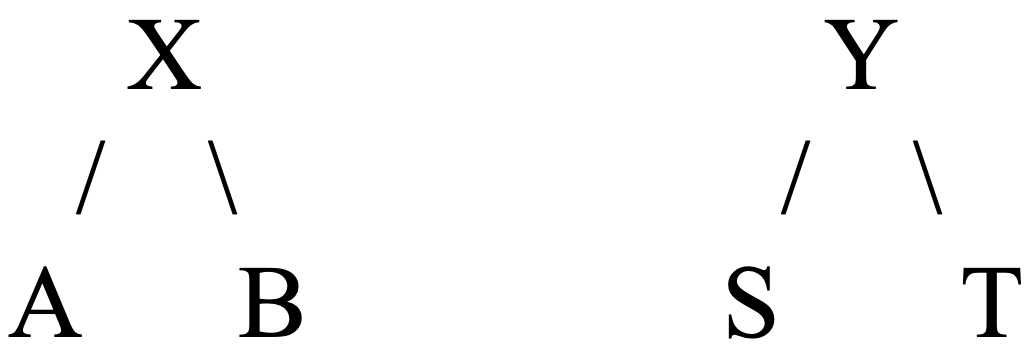
\includegraphics[width=0.4\linewidth]{images/HL1.png}
        \end{figure}
        Given the resource hierarchy above, is the following schedule compatible with a 2PL-strict scheduler that applies hierarchical locking?
        \[r_1(A) w_1(S) w_2(T) r_2(A) w_1(A)\]
    \subsection*{Solution}
        The lock manager works as follows: 
        \begin{table}[H]
            \centering
            \begin{tabular}{c|cccccc|c}
            \cline{2-7}
            \textit{}                          & \textit{X}               & \textit{A}              & \textit{B} & \textit{Y}               & \textit{S}          & \textit{T}          & \textit{}    \\ \cline{1-7}
            \multicolumn{1}{|c|}{$r_1(A)$}     & $\textnormal{ISL}_1$     & -                       & -          & -                        & -                   & -                   &              \\
            \multicolumn{1}{|c|}{}             & $\textnormal{ISL}_1$     & $\textnormal{SL}_1$     & -          & -                        & -                   & -                   &              \\
            \multicolumn{1}{|c|}{$w_1(S)$}     & $\textnormal{ISL}_1$     & $\textnormal{SL}_1$     & -          & $\textnormal{IXL}_1$     & -                   & -                   &              \\
            \multicolumn{1}{|c|}{}             & $\textnormal{ISL}_1$     & $\textnormal{SL}_1$     & -          & $\textnormal{IXL}_1$     & $\textnormal{XL}_1$ & -                   &              \\
            \multicolumn{1}{|c|}{$w_2(T)$}     & $\textnormal{ISL}_1$     & $\textnormal{SL}_1$     & -          & $\textnormal{IXL}_{1,2}$ & $\textnormal{XL}_1$ & -                   &              \\
            \multicolumn{1}{|c|}{}             & $\textnormal{ISL}_1$     & $\textnormal{SL}_1$     & -          & $\textnormal{IXL}_{1,2}$ & $\textnormal{XL}_1$ & $\textnormal{XL}_2$ &              \\
            \multicolumn{1}{|c|}{$r_2(A)$}     & $\textnormal{ISL}_{1,2}$ & $\textnormal{SL}_1$     & -          & $\textnormal{IXL}_{1,2}$ & $\textnormal{XL}_1$ & $\textnormal{XL}_2$ &              \\
            \multicolumn{1}{|c|}{}             & $\textnormal{ISL}_{1,2}$ & $\textnormal{SL}_{1,2}$ & -          & $\textnormal{IXL}_{1,2}$ & $\textnormal{XL}_1$ & $\textnormal{XL}_2$ &              \\
            \multicolumn{1}{|c|}{commit $T_2$} &                          &                         &            &                          &                     &                     & End of $T_2$ \\
            \multicolumn{1}{|c|}{}             & $\textbf{ISL}_1$         & $\textnormal{SL}_1$     & -          & $\textnormal{IXL}_1$     & $\textnormal{XL}_1$ & -                   &              \\
            \multicolumn{1}{|c|}{$w_1(A)$}     & $\textbf{IXL}_1$         & $\textbf{SL}_1$         & -          & $\textnormal{IXL}_1$     & $\textnormal{XL}_1$ & -                   &              \\
            \multicolumn{1}{|c|}{}             & $\textnormal{IXL}_1$     & $\textbf{XL}_1$         & -          & $\textnormal{IXL}_1$     & $\textnormal{XL}_1$ & -                   &              \\
            \multicolumn{1}{|c|}{commit $T_1$} &                          &                         &            &                          &                     &                     & End of $T_1$ \\ \cline{1-7}
            \end{tabular}
        \end{table}
        So, it is compatible with a strict 2PL scheduler. 

    \newpage

    \section{Hierarchical lock}
        Consider the following short schedule occurring on a system with hierarchical lock over a hierarchy where $PagA$ contains tuples 
        $t_1$ and $t_2$:
        \[r_1( PagA ), w_2( t1 ), w_1( t2 )\]
        Show a possible sequence of locks, unlocks, lock upgrades, and lock downgrades performed by transactions $T_1$ and $T_2$ such that
        the schedule is in 2PL.
    \subsection*{Solution}
        We have that: 
        \begin{table}[H]
            \centering
            \begin{tabular}{c|ccc|}
            \cline{2-4}
            \textit{}                    & \textbf{PagA}                           & \textbf{t2}          & \textbf{t1}           \\ \cline{2-4} 
            $\textnormal{SIXL}_1(PagA)$  & $\textnormal{SIXL}_1$                   & -                    & -                     \\
            $\textnormal{XL}_1(t2)$      & $\textnormal{SIXL}_1$                   & $\textnormal{XL}_1$  & -                     \\
            $r_1(PagA)$                  &                                         &                      &                       \\
            $\textnormal{U-SL}_1(PagA)$  & $\textnormal{IXL}_1,\textnormal{IXL}_2$ & $\textnormal{XL}_1$  & -                     \\
            $\textnormal{IXL}_2(PagA)$   & $\textnormal{IXL}_1,\textnormal{IXL}_2$ & $\textnormal{XL}_1$  & -                     \\
            $\textnormal{XL}_2(t1)$      & $\textnormal{IXL}_1,\textnormal{IXL}_2$ & $\textnormal{XL}_1$  & $\textnormal{XL}_2$   \\
            $w_2(t1)$                    &                                         &                      &                       \\
            $\textnormal{U-XL}_2(t1)$    & $\textnormal{IXL}_1,\textnormal{IXL}_2$ & $\textnormal{XL}_1$  & -                     \\
            $\textnormal{U-IXL}_2(PagA)$ & $\textnormal{IXL}_1$                    & $\textnormal{XL}_1$  & -                     \\
            Commit $T_2$                 &                                         &                      &                       \\
            $w_1(t2)$                    &                                         &                      &                       \\
            $\textnormal{U-XL}_1(t2)$    & $\textnormal{IXL}_1$                    & -                    & -                     \\
            $\textnormal{U-IXL}_1(PagA)$ & -                                       & -                    & -                     \\
            Commit $T_1$                 & \multicolumn{1}{l}{}                    & \multicolumn{1}{l}{} & \multicolumn{1}{l|}{} \\ \cline{2-4} 
            \end{tabular}
        \end{table}
        So the schedule is 2PL.

    \newpage 

    \chapter{Exercise session IV}
\end{document}